% ============================================================================================
% Draft methods and results for the full-state teachers and the ICL transformer (Nathan).
% Meant to be \input into the team's NeurIPS-style paper. Needs: amsmath, amssymb, booktabs,
% graphicx, xcolor, algorithm + algpseudocode (or drop the algorithm block).
% Figures: upload state_bc/results/transformer_v1_seed0/figures/*.pdf to figures/ in Overleaf;
% they are regenerated by `python state_bc/make_figures.py`.
% Lines marked %CHECK need a team member to confirm a fact before submission.
% ============================================================================================

\providecommand{\inprogress}[1]{\textcolor{red}{[In progress: #1]}}

\section{Method}
\label{sec:method}

\subsection{Task: Push-T with a hidden goal}
\label{sec:task}
We use \texttt{PushTVarGoal-v1}, a variable-goal version of ManiSkill's \texttt{PushT-v1}~\cite{tao2024maniskill3}
(the Push-T task originates in~\cite{florence2021implicit}), written by Jimmy (Section~\ref{sec:ppo}). A Panda arm with a stick
end-effector pushes a T-shaped block on a table to a goal pose. The full state $s_t \in \mathbb{R}^{31}$ contains joint positions and
velocities, the tool-tip pose, the goal position $g$ (3 numbers) and the T's pose. Actions $a_t \in [-1,1]^7$ are joint-position
deltas (\texttt{pd\_joint\_delta\_pos}), and an episode lasts $T = 100$ steps.

\textbf{Goals and quadrants.} Each episode samples a goal position from one of four quadrants $Q_1,\dots,Q_4$ around a fixed
origin: $\pm 10$\,cm in $x$ and $\pm 20$\,cm in $y$, with a 2--3\,cm band around each axis excluded so the quadrants are
separated. The goal orientation is fixed. %CHECK quadrant numbering convention and which axis has the 2 vs 3 cm band
The T starts 8--30\,cm from the goal, and the arm starts from one of 600 precomputed poses.

\textbf{Hiding the goal.} The goal-conditioned teachers (Section~\ref{sec:teachers}) see $s_t$. The transformer only sees
$\phi(s_t) \in \mathbb{R}^{28}$, the state with the goal removed. Within an episode the goal is constant, so the only way the
transformer can learn where to push is from the demonstrations in its prompt.

\textbf{Metrics.} An episode is a success at step $t$ when the T overlaps the goal pose closely enough under ManiSkill's
\texttt{PushT-v1} criterion. %CHECK state the exact threshold
We report \emph{success-once} (success at any step) and \emph{success-at-end} (success at the final step). The gap between them
measures whether a policy that reaches the goal also stops there.

\subsection{Goal-conditioned teachers}
\label{sec:teachers}

\textbf{PPO teacher} (Jimmy; Section~\ref{sec:ppo}). A goal-conditioned PPO~\cite{schulman2017ppo} policy trained for 50M
environment steps with ManiSkill's PPO baseline on goals from all four quadrants. We use its deterministic (mean) action.
%CHECK with Jimmy: training details; sec:ppo is the label of his section

\textbf{BC teacher, distilled from PPO.} We distill the frozen PPO teacher into an MLP
$\pi_{\mathrm{BC}}: \mathbb{R}^{31} \to [-1,1]^7$ (two hidden layers of 256 units, ReLU, $\tanh$ output). To avoid the compounding
errors of plain behavior cloning~\cite{ross2011dagger}, the training states come from \emph{noisy} teacher rollouts. A Gaussian
perturbation $\epsilon \sim \mathcal{N}(0,\sigma^2 I)$ with $\sigma \in \{0, 0.1, 0.2, 0.3\}$ (cycled across batches) is added to
the executed action, while the label is always the teacher's clean action $\pi_{\mathrm{PPO}}(s_t)$, as in DART~\cite{laskey2017dart}.
We collect 16{,}384 episodes (1.64M transitions) on goals in all four quadrants and minimize the mean squared action error with Adam
(learning rate $3\times10^{-4}$, cosine decay, batch 1{,}024, 200k steps). We do not use DAgger: in an earlier fixed-goal experiment
(Appendix~\ref{app:teacher-history}) it added nothing measurable over noise injection.

\textbf{Teacher quality.} On 100 test episodes per quadrant (seeds fixed per quadrant), the PPO teacher scores 93.8\% / 91.5\% mean
success-once / success-at-end and the BC teacher 91.5\% / 88.8\%. Both reach at least 89\% success-once in every quadrant, including $Q_4$.
A transformer failure on $Q_4$ goals is therefore not explained by weak teachers there.
Both teachers see $Q_4$ goals in training. Only the transformer is restricted to $Q_1$--$Q_3$.

\subsection{Demonstration data}
\label{sec:data}
For each split we draw a fixed set of goal positions from its quadrants, independently and with its own seed
(Table~\ref{tab:splits}). For each goal and teacher we roll out 10 noise-free episodes from different initial states, recording
$(\phi(s_t), a_t)$ for all 100 steps. The goal is recorded only to group episodes by goal and is never given to the model.
Test goals are new positions: none appears in training.

\begin{table}[h]
\centering
\caption{Goal splits for the transformer. Each goal has 10 demonstrations per teacher. Teacher columns give the success-once /
success-at-end of those demonstrations (\%).}
\label{tab:splits}
\begin{tabular}{lccccc}
\toprule
Split & Quadrants & Goals & Demos (both teachers) & PPO demos & BC demos \\
\midrule
train & $Q_1$--$Q_3$ & 2{,}048 & 40{,}960 & 93.8 / 89.3 & 93.1 / 86.8 \\
val & $Q_1$--$Q_3$ & 128 & 2{,}560 & 93.5 / 87.1 & 92.2 / 84.8 \\
test (in distribution) & $Q_1$--$Q_3$ & 128 & 2{,}560 & 94.1 / 91.1 & 93.4 / 87.7 \\
test (held out) & $Q_4$ & 128 & 2{,}560 & 94.5 / 93.4 & 92.7 / 90.5 \\
\bottomrule
\end{tabular}
\end{table}

\subsection{In-context transformer}
\label{sec:icl-model}

\textbf{Prompt.} Following the function-class setup of Garg et al.~\cite{garg2022can}, a prompt contains examples of a hidden
``task'' followed by a query. Here the task is a goal, and the examples are $k$ whole demonstrations of it by one teacher.
Each demonstration $j$ is subsampled every $r = 4$ steps, keeping the last step so the final T pose is included:
$\mathcal{S} = \{T-1, T-1-r, \dots\}$, which gives $P = |\mathcal{S}| = 25$ state--action pairs. With demonstrations
$\tau^1,\dots,\tau^k$ of goal $g$ by teacher $m$, the prompt is
\begin{equation}
  X_k = \big(\phi(s^1_{t}), a^1_{t}\big)_{t \in \mathcal{S}},\ \dots,\ \big(\phi(s^k_{t}), a^k_{t}\big)_{t \in \mathcal{S}},\ \phi(s^q),
  \label{eq:prompt}
\end{equation}
one token per state and per action, so $2kP + 1$ tokens ($401$ at $k = 8$). The query state $s^q$ is a uniformly random step of a
\emph{different} demonstration $\tau^q$ of the same goal and teacher; its label is the teacher's action $a^q$ there.

\textbf{Architecture.} States and actions are embedded by separate linear maps,
$e(s) = W_s\,(\phi(s) - \mu)/\sigma$ and $e(a) = W_a\,a$, where $\mu, \sigma$ are per-dimension training-set statistics. The token
sequence goes through a causal GPT-2 backbone~\cite{radford2019gpt2} with learned absolute position embeddings: 12 layers, width 256,
8 heads and no dropout, 9.75M parameters in total. A linear head reads the last hidden state,
$\hat a = W_o\, h_{2kP+1}$. Unlike Garg et al., who predict at every query position, we predict only at the final token.

\textbf{Training objective.} Each step samples one context size $k$ uniformly from $\{0,1,2,4,8\}$ and then, for each of 64
prompts, a teacher $m$ and a training goal $g$ uniformly. Within a goal, demonstrations are ordered successful-first (random
otherwise), the first $k$ form the support and the next one supplies the query. We minimize
\begin{equation}
  \mathcal{L}(\theta) = \mathbb{E}_{k,\,m,\,g,\,\tau^{1:k},\,\tau^q,\,t}\,
  \big\| f_\theta(X_k) - a^q_t \big\|_2^2 .
  \label{eq:loss}
\end{equation}
At $k = 0$ the prompt is only $\phi(s^q)$, so the model must output a goal-independent action. That gives the no-context baseline.
Table~\ref{tab:hparams} lists the hyperparameters. The architecture, learning rate and batch size follow Garg et al.~\cite{garg2022can}
and were not tuned. %CHECK: confirm Garg et al. use 12 layers / 256 / 8 heads, lr 1e-4, batch 64

\begin{table}[h]
\centering
\caption{Transformer hyperparameters. Nothing was tuned on test data. The only earlier run is a 3k-step pilot with the same settings.}
\label{tab:hparams}
\begin{tabular}{lll}
\toprule
Setting & Value & Reason \\
\midrule
Layers / width / heads & 12 / 256 / 8 & GPT-2 setup of~\cite{garg2022can} \\
Optimizer & AdamW~\cite{loshchilov2019adamw}, lr $10^{-4}$, no weight decay & lr as in~\cite{garg2022can} \\
Batch size & 64 prompts & as in~\cite{garg2022can} \\
Schedule & 1k-step linear warmup, cosine~\cite{loshchilov2017sgdr} to 10\% & standard; not tuned \\
Training steps & 100k & compute budget (3.6\,h on one L4); val.\ loss still decreasing \\
Context sizes $k$ & $\{0,1,2,4,8\}$, uniform & no context up to 8 demos \\
Subsampling stride $r$ & 4 (25 pairs per demo) & $k = 8$ fits in 1{,}024 positions \\
Precision & bf16 autocast, gradient clip 1.0 & speed \\
Checkpoint selection & lowest val.\ MSE averaged over $k$ (correct goal) & selected the final step \\
\bottomrule
\end{tabular}
\end{table}

\subsection{Evaluation}
\label{sec:eval}
All evaluation uses the frozen checkpoint and goals the transformer never trained on.

\textbf{Controls.} The design has to show that success comes from reading the context. We therefore evaluate every setting under
three conditions:
\begin{itemize}
  \item \emph{correct goal}: demonstrations of the evaluation goal;
  \item \emph{wrong goal}: demonstrations of a different goal from the same split, with everything else identical;
  \item \emph{no demos}: $k = 0$.
\end{itemize}
A model that ignores its context scores the same under all three.

\textbf{Teacher-forced action error.} For each split and $k$, the mean squared error of $\hat a$ on 1{,}024 sampled prompts.
The correct- and wrong-goal conditions use the same queries.

\textbf{Closed-loop success.} For each split we take 128 goals and 4 new initial states per goal, 512 episodes per condition. The
support for goal $g$ is fixed: the first $k$ demonstrations of $g$ (successful first) collected by the context teacher. Every
condition, including the two goal-seeing teachers, runs from the \emph{same} 512 initial states, so differences between conditions
are paired. Wrong-goal episodes use the support of goal $(g + 64) \bmod 128$.

\begin{algorithm}[h]
\caption{Closed-loop evaluation of one condition (vectorized over the 512 episodes in practice)}
\label{alg:closed-loop}
\begin{algorithmic}[1]
\Require frozen $f_\theta$; support $D$ of $k$ subsampled demonstrations (Eq.~\ref{eq:prompt}); goal $g$; initial-state seed
\State $s_0 \gets \textsc{Reset}(g, \text{seed})$ \Comment{same seed for every condition}
\For{$t = 0, \dots, T-1$}
  \State $a_t \gets \mathrm{clip}\big(f_\theta(D, \phi(s_t)),\, -1,\, 1\big)$ \Comment{the goal is never an input}
  \State $s_{t+1} \gets \textsc{Step}(s_t, a_t)$; record whether the episode is a success at $t+1$
\EndFor
\State \Return success-once, success-at-end
\end{algorithmic}
\end{algorithm}

\textbf{Uncertainty.} Success rates come with 95\% Wilson score intervals~\cite{wilson1927probable} for a binomial proportion over
$n = 512$ episodes: about $\pm 3$ points near 90\% and $\pm 4$ near 65\%. These intervals treat episodes as independent. They ignore
that the 4 episodes of a goal share it, and they do not capture variation across training seeds.
\inprogress{only one training seed so far; seeds 1--2 will give between-seed error bars.}
\inprogress{a goal-estimate baseline: estimate $g$ from the final T pose in the demonstrations and give it to the BC teacher.}

% ============================================================================================
\section{Results}
\label{sec:results}

\subsection{The transformer learns to use its context}
Figure~\ref{fig:training} shows training. With correct-goal demonstrations, validation error at $k = 4$ falls from 0.015 to 0.0015,
while error with wrong-goal demonstrations \emph{rises} from 0.020 to 0.14 over the same steps. The model becomes more committed to
the goal its context implies, even when that goal is wrong. The no-demo error levels off at 0.0044, which is the best a policy can do
without knowing the goal, about $3\times$ the correct-goal error. The checkpoint with the lowest validation error was the final one
(step 100k), and validation error was still falling slowly, so longer training might help.

\begin{figure}[h]
  \centering
  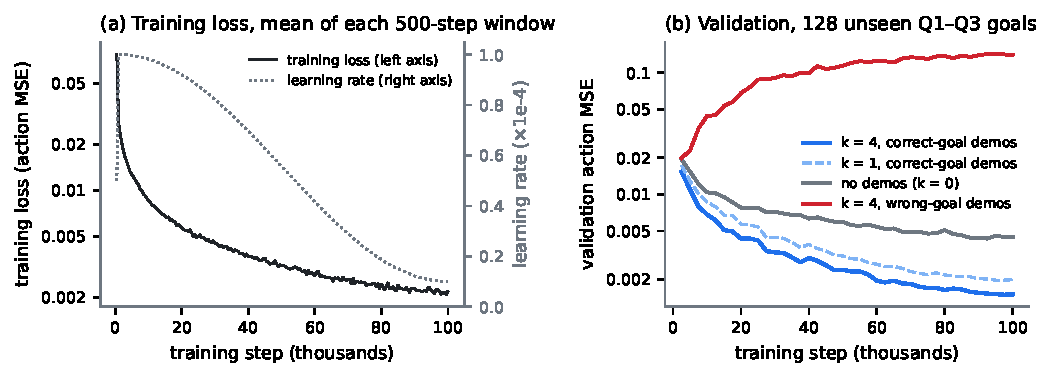
\includegraphics[width=\linewidth]{figures/fig_training.pdf}
  \caption{\textbf{Training.} (a) Training loss (mean over 500-step windows, all $k$ mixed) and the learning-rate schedule.
  (b) Validation action MSE on 128 unseen $Q_1$--$Q_3$ goals, evaluated every 2{,}500 steps. Log scale because the errors span two
  orders of magnitude. Wrong-goal error grows as the model learns to rely on the context.}
  \label{fig:training}
\end{figure}

\subsection{In distribution, in-context control matches the teachers}
Table~\ref{tab:main} gives closed-loop success at $k = 4$. On unseen $Q_1$--$Q_3$ goals, the transformer reaches 91.2\% / 87.5\%
success-once / at-end with PPO demonstrations and 91.6\% / 87.5\% with BC demonstrations. That is within the confidence intervals
of the teachers that see the goal (94.1\% / 89.1\% and 92.0\% / 85.9\%). Under the controls it collapses: 1.4--1.6\% success-once
with wrong-goal demonstrations and 0.8--1.4\% with none. Every condition runs from the same initial states, so the gap of about
90 points is caused by the content of the context alone.

\begin{table}[h]
\centering
\caption{\textbf{Closed-loop success at $k = 4$} (\%; 512 episodes per cell, 95\% Wilson interval in brackets). All conditions in
a row use the same initial states.}
\label{tab:main}
\small
\begin{tabular}{lllcccc}
\toprule
Goals & Demos & Metric & Correct goal & Wrong goal & No demos & Teacher (sees $g$) \\
\midrule
$Q_1$--$Q_3$ & PPO & once   & 91.2 [88.4, 93.4] & 1.4 [0.7, 2.8] & 1.4 [0.7, 2.8] & 94.1 [91.8, 95.9] \\
             &     & at end & 87.5 [84.4, 90.1] & 1.0 [0.4, 2.3] & 0.4 [0.1, 1.4] & 89.1 [86.1, 91.5] \\
             & BC  & once   & 91.6 [88.9, 93.7] & 1.6 [0.8, 3.1] & 0.8 [0.3, 2.0] & 92.0 [89.3, 94.0] \\
             &     & at end & 87.5 [84.4, 90.1] & 0.8 [0.3, 2.0] & 0.4 [0.1, 1.4] & 85.9 [82.7, 88.7] \\
\midrule
$Q_4$ (held out) & PPO & once   & 86.1 [82.9, 88.9] & 3.9 [2.5, 6.0] & 0.2 [0.0, 1.1] & 94.7 [92.4, 96.4] \\
                 &     & at end & 67.0 [62.8, 70.9] & 0.0 [0.0, 0.7] & 0.0 [0.0, 0.7] & 92.6 [90.0, 94.5] \\
                 & BC  & once   & 88.5 [85.4, 91.0] & 3.5 [2.2, 5.5] & 0.2 [0.0, 1.1] & 94.9 [92.7, 96.5] \\
                 &     & at end & 63.7 [59.4, 67.7] & 0.4 [0.1, 1.4] & 0.0 [0.0, 0.7] & 93.6 [91.1, 95.4] \\
\bottomrule
\end{tabular}
\end{table}

\textbf{PPO and BC demonstrations are interchangeable.} The same model reaches the same success with either teacher's demonstrations
(Table~\ref{tab:main}, Figure~\ref{fig:k}). This is expected, since the BC teacher imitates the PPO teacher. It also means the teacher
mixture adds little variety. Goal variety does the work.

\subsection{One demonstration is nearly enough}
Figure~\ref{fig:k} varies $k$. A single demonstration already gives 90--91\% success-once on $Q_1$--$Q_3$, and $k \ge 2$ mainly
improves success-at-end (82--84\% at $k = 1$, 88\% at $k = 2$). Beyond $k = 2$ the curves are flat within their intervals. This fits
the task: the goal is a 2-D position, and one successful demonstration shows where the T ended up, which is almost the goal itself.
We return to this in Section~\ref{sec:limitations}.
Teacher-forced error is lowest at $k = 4$ and slightly higher at $k = 8$, most clearly on $Q_4$ (0.0041 vs 0.0027;
Appendix Table~\ref{tab:action-error}). The difference does not appear in closed loop. One possible reason is that each $k$ gets a
fifth of the training steps, so the position embeddings used only by $k = 8$ prompts (positions 201--400) are trained on the fewest
prompts. We have not tested this.

\begin{figure}[h]
  \centering
  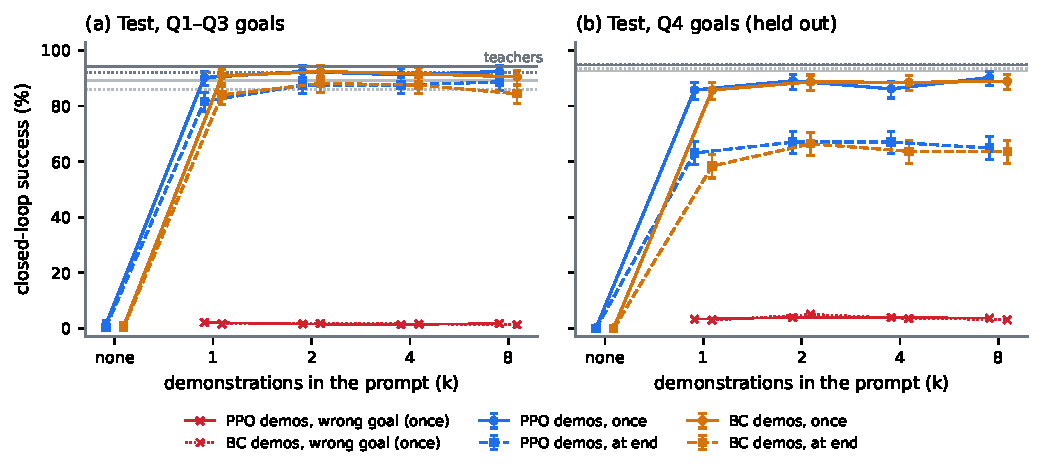
\includegraphics[width=\linewidth]{figures/fig_success_vs_k.pdf}
  \caption{\textbf{Closed-loop success vs number of demonstrations $k$} for unseen in-distribution goals (a) and held-out $Q_4$
  goals (b). Solid: success-once; dashed: success-at-end; red: wrong-goal demonstrations; grey lines: the goal-seeing teachers
  (solid PPO, dotted BC; darker once, lighter at end). Error bars are 95\% Wilson intervals over 512 episodes (one training seed).
  Points for PPO and BC demonstrations are offset slightly in $x$ for readability.}
  \label{fig:k}
\end{figure}

\subsection{Held-out goals: reaching transfers, holding does not}
On $Q_4$ goals, which the transformer never trained on, the controls still behave as before: at most 3.9\% with wrong-goal
demonstrations and 0.2\% with none. The model reads held-out goals from its context. Success-once stays high (86.1--88.5\%, against
94.7--94.9\% for the teachers), but success-at-end drops to 63.7--67.0\% against the teachers' 92.6--93.6\%. In distribution, the
transformer loses about 4 points between success-once and success-at-end; on $Q_4$ it loses 19--25. So in roughly a quarter of
$Q_4$ episodes it brings the T onto the goal and then pushes it off again. Extra demonstrations do not fix this: success-at-end
levels off at 64--67\% from $k = 2$ (Figure~\ref{fig:k}b). Teacher-forced error tells the same story: 0.0027 on $Q_4$ against 0.0016 in
distribution at $k = 4$. That is still 3$\times$ better than no context, but enough to matter for fine positioning. Our reading:
the coarse behavior, pushing toward the goal the context implies, generalizes to new goal positions. The precise corrective
actions near an unfamiliar goal do not.

\subsection{Offline error has a closed-loop threshold}
A 3k-step pilot with the same settings reached validation action MSE 0.013 at $k = 4$ and already preferred correct over wrong
demonstrations (0.013 vs 0.016). In closed loop, however, it scored 0\% on 64 validation goals $\times$ 2 starts under every
condition, while the teachers scored 91--94\% on the same starts. At 0.0015 the final model matches the teachers. Small per-step
errors compound over 100 steps, so teacher-forced error is informative only once it is small. Closed-loop evaluation is necessary.

\subsection{Comparison with an independent implementation}
\label{sec:compare}
Jimmy independently trained the same architecture on the same teachers, goal splits and closed-loop protocol, in a separate
codebase, for 50k steps at a constant learning rate in fp16 (two seeds). Teacher success on the evaluation starts matches exactly,
so the closed-loop numbers are directly comparable (Table~\ref{tab:compare}). Both runs show the same qualitative results: success
comes from the context, about 0\% under both controls, $k = 1$ gives most of the effect, PPO and BC demonstrations are
interchangeable, and $Q_4$ success-at-end drops. Our run is stronger: success-once is 8 points higher and success-at-end 20 points
higher in distribution, consistent with its roughly $3\times$ lower action error.

\textbf{This comparison is not controlled.} Training length, learning-rate schedule, numeric precision and code all differ at once,
so we cannot attribute the gap to one of them. At 50k steps, the same number Jimmy trained for, our validation error was already 0.0024, below his
final 0.004--0.006. That suggests the decaying learning rate matters, not only the extra steps. A one-factor test is to rerun his code
with our schedule. Jimmy's two seeds also differ by 31 points in $Q_4$ success-at-end (41\% vs 72\%, PPO demos, $k = 4$), while
success-once is stable (77\% vs 79\%). Our single-seed $Q_4$ success-at-end therefore has wide uncertainty beyond the binomial
interval in Table~\ref{tab:main}. Success-once and the in-distribution results look stable.

\begin{table}[h]
\centering
\caption{Our run vs.\ Jimmy's independent run at $k = 4$ (success-once / at-end, \%). The rows differ in several settings at once
(see text).}
\label{tab:compare}
\small
\begin{tabular}{lcccc}
\toprule
Run & Steps, schedule & Val.\ MSE (correct) & $Q_1$--$Q_3$, PPO demos & $Q_4$, PPO demos \\
\midrule
Ours (1 seed) & 100k, warmup + cosine & 0.0015 & 91.2 / 87.5 & 86.1 / 67.0 \\
Jimmy (mean of 2 seeds) & 50k, constant & 0.004--0.006 & 83 / 68 & 78 / 56 \\
\bottomrule
\end{tabular}
\end{table}

\subsection{Limitations}
\label{sec:limitations}
\begin{itemize}
  \item \textbf{One training seed.} The $Q_4$ success-at-end figure in particular needs more seeds. \inprogress{seeds 1 and 2.}
  \item \textbf{Goal inference may be simple.} A successful demonstration's final T pose nearly reveals the 2-D goal, so the model may
    be doing little more than reading where the T ended up. That is still in-context inference of a hidden task variable, but a
    simple form. The goal-estimate baseline (Section~\ref{sec:eval}) will show how much more the transformer does. \inprogress{baseline.}
  \item \textbf{$Q_4$ is closer to recombination than extrapolation.} Each coordinate's sign appears in $Q_1$--$Q_3$; only the
    combination is new.
  \item \textbf{Noise-free demonstrations only.} Every demonstration and query state comes from clean teacher rollouts. The holding
    failure on $Q_4$ may come partly from never training on states near the goal that the teachers themselves avoid. Training on
    queries from noisy rollouts with clean labels, as for the BC teacher, is the obvious next experiment.
\end{itemize}

% ============================================================================================
\appendix
\section{Teacher-forced action error}
\label{app:action-error}
\begin{table}[h]
\centering
\caption{Teacher-forced action MSE of the selected checkpoint (correct-goal / wrong-goal demonstrations; 1{,}024 prompts per cell).}
\label{tab:action-error}
\small
\begin{tabular}{lccccc}
\toprule
Split & no demos & $k{=}1$ & $k{=}2$ & $k{=}4$ & $k{=}8$ \\
\midrule
val ($Q_1$--$Q_3$) & 0.0045 & 0.0019 / 0.117 & 0.0017 / 0.128 & 0.0015 / 0.135 & 0.0017 / 0.127 \\
test ($Q_1$--$Q_3$) & 0.0044 & 0.0020 / 0.125 & 0.0017 / 0.137 & 0.0016 / 0.142 & 0.0018 / 0.134 \\
test ($Q_4$) & 0.0076 & 0.0031 / 0.077 & 0.0029 / 0.082 & 0.0027 / 0.088 & 0.0041 / 0.085 \\
\bottomrule
\end{tabular}
\end{table}
Wrong-goal error is lower on $Q_4$ because the wrong goal is another $Q_4$ goal, closer on average than goals spread over three quadrants.

\section{Development history of the BC teacher}
\label{app:teacher-history}
\inprogress{short summary of runs 1--3 from \texttt{state\_bc/README.md}. Run 1 used plain BC on released demonstrations (19\% / 10\%
success); run 2 added noisy expert rollouts and DAgger (98\% / 78\%, with DAgger adding nothing measurable); run 3 trained our own
variable-goal environment and PPO, then the team adopted Jimmy's shared environment.}
